\section{Rupture Optimizations}\label{subsec:optimizations}

\subsection{Block alignment}\label{subsec:blockalign}
Block ciphers are \textit{length monotonic}, but not \textit{strictly length
monotonic}, as described in section \ref{subsec:lenmonotone}. Specifically, the
length of the encrypted text is rounded up to a product of $\mu$-bits, where $\mu$
is the block size, using added padding. The same applies for stream ciphers,
whose functionality is similar to block ciphers with block size 1 byte. In this
case, plaintext length difference between two messages does not always result in
length difference between the respective encrypted ciphertext.

It is possible to bypass this problem by using block alignment. Block alignment
techniques have already been explored in the literature \cite{moller2014poodle}. This method
demands issuing multiple requests to the reflection oracle while including
artificial noise in the reflection string $r$.

In each request $r_{i, c}$ for each candidate $c$ in the secret alphabet, we add
increasing artificial noise. That way, all $r_{1, c}$ for all c in candidates
will contain one character of alignment noise, $r_{2, c}$ will contain two
characters and so forth. As mentioned above, the difference in length of the
compressed plaintext for the correct candidate and an incorrect one is 1 byte.
For some alignment noise length $a \in [0, \mu)$ the reflection of the correct
candidate will be $(\delta*\mu)$ and for all incorrect candidates
$(\delta*\mu)+1$. In that case, the incorrect candidates result in one more
block over the network compared to the correct one.  This ensures that one out
of $\ceil{\mu / |r_i|}$ requests will result in a block distinction between the
alphabet candidates.

Figure \ref{fig:block_alignment} intuitively depicts the block alignment technique.

   \begin{figure}[thpb]
      \centering
          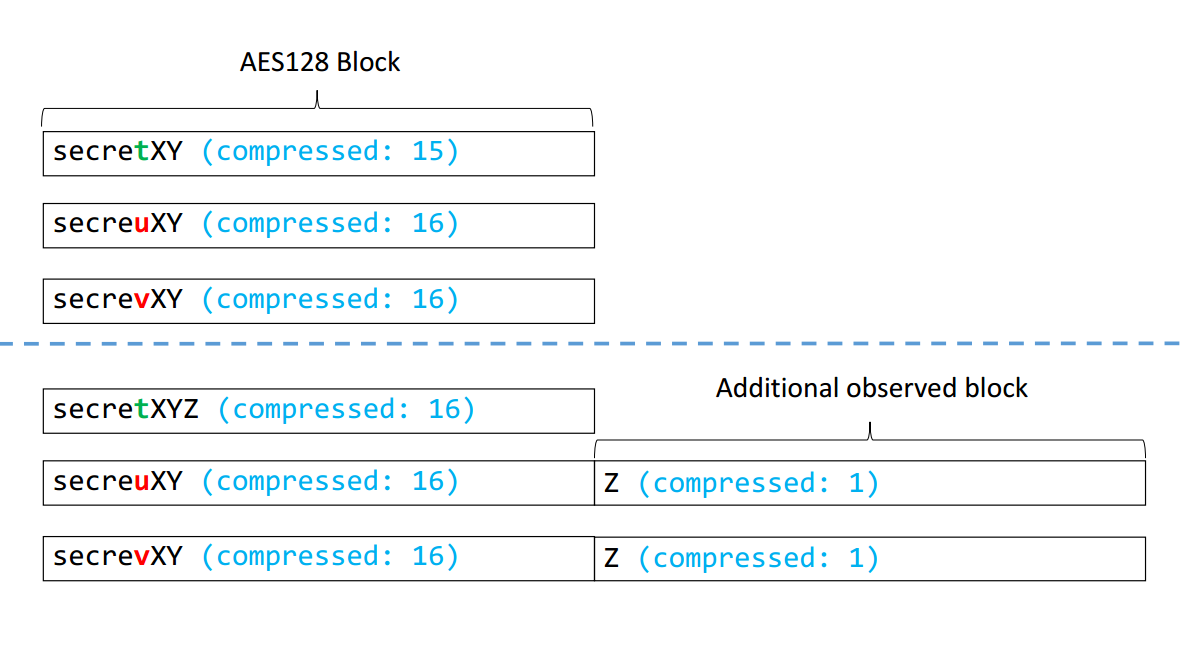
\includegraphics[width=0.48\textwidth]{figures/block_alignment.png}
      \caption{The block alignment method}
      \label{fig:block_alignment}
   \end{figure}

\subsection{Reflection computation methods}\label{subsec:reflectionmethods}
The reflection strings $r$ should be polynomially computable, as defined in
\ref{sec:propertycom}. BREACH is
parameterized with an alphabet of ASCII symbols $\Sigma$
for each character of the
secret. A successful attack should distinguish a single character of the
alphabet as the correct one through a series of requests to the reflection
oracle.

The first method of issuing requests is serial. Each request to the oracle
corresponds to a single character of the alphabet. An attack phase is completed
when requests have been issued for the entire alphabet.

In this case, $Q$ is the predicate "Given a known prefix $p_s$ of secret $s$ and
a symbol $t \in \Sigma$, is $p_s || t$ a prefix of $s$?". The complexity of the attack is $\mathcal{O}(|\Sigma|)$ and
the round ends by finding a character of the secret. This method is similar to
how BREACH previously worked.

The second method of attack is divide and conquer. In each phase the alphabet is
divided into two subsets $\Sigma_1$ and $\Sigma_2 =
\Sigma
\setminus \Sigma_1$, where $|\Sigma_1| = |\Sigma_2| =
\ceil{|\Sigma| / 2}$. The reflection string for $\Sigma_1$ consists of
$|\Sigma_1|$ substrings divided by an annotation symbol $\beta$ which is not
present in the regular plaintext. Each
substring consists of the known part of the secret concatenated with a character
in $\Sigma_1$. The reflection string for $\Sigma_2$ is constructed
similarly. For example, if $\Sigma_1$ is $\{"1", "2"\}$ and the known prefix is
"abc", using "-" as $\beta$ the reflection is: "abc1-abc2".
Each phase consists of one call to the reflection oracle per subset.

The predicate $Q$ in this case is "Given a known prefix $p_s$ of the secret $s$, is
$p_s || t$ a
prefix of $s$, where $t \in \Sigma_1$?". As long as the prefix of the
secret is \textit{compression-detectable} by each substring of the reflection,
the end of each phase marks the choice of subset $\Sigma_i$ that contains
the correct alphabet symbol and the same method is applied using chosen
$\Sigma_i$ as the alphabet $\Sigma$. The round is complete when
$|\Sigma| = 1$. Each round reduces the alphabet by half, so the complexity
of the attack with the divide and conquer method  is
$\mathcal{O}(log|\Sigma|)$.

Figure \ref{fig:divide_and_conquer} shows the reflection sequence for the case
when the alphabet is the number digits. In order to find the correct leaf of the
tree, we construct two reflections in each round. The two reflections contain
the children nodes of the parent node that was chosen in the previous round,
beginning with the root of the tree. After traversing the tree, we reach the
correct choice which is number 3.

   \begin{figure}[thpb]
      \centering
          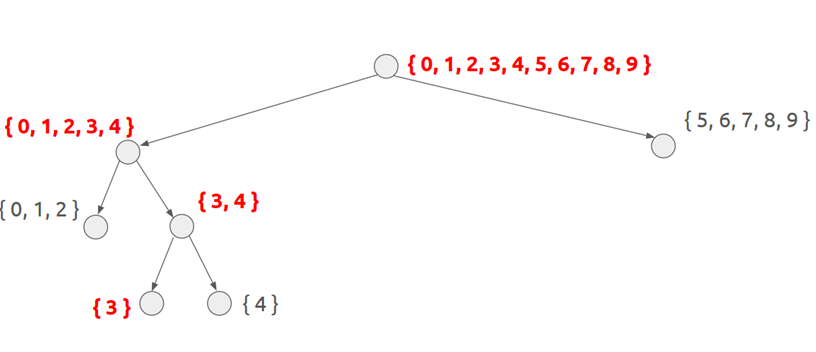
\includegraphics[width=0.48\textwidth]{figures/divide_and_conquer.png}
      \caption{The divide \& conquer method}
      \label{fig:divide_and_conquer}
   \end{figure}

\subsection{Request parallelization}\label{subsec:parallel}
The reflection oracle is generally considered synchronous. However, this is not
always the case, since it may be able to handle multiple parallel requests from
the adversary.

This is the case for the oracle in BREACH. Here the reflection oracle is an endpoint
offered by a web application and the communication channel between the adversary
and the oracle is the end-to-end browser-server network channel.

Modern web servers are able to handle multiple parallel requests and
browsers can issue a certain amount of parallel requests per domain. This
functionality enables the adversary to issue multiple parallel requests per
symbol in alphabet $\Sigma$ and efficiently reduce the execution time of
the attack.

\subsection{Request soup}
Previous sections demonstrated the need for multiple requests per reflection
string $r_i$. However, it is often the case that communication with the
reflection oracle is time
expensive. In this case, it is preferable to issue multiple
requests for a candidate and treat them as a set rather than separately.

This technique is useful in the case of BREACH. Communication between the browser and the
endpoint is encrypted, so the time needed for the analysis of
the captured packets depends on the request set.

A request set consists of requests for a symbol $s_i$ in alphabet
$\Sigma$.
Bigger request sets result in less time delay. Length calculation per request
can then be measured as the mean length over the number of requests in the set.

This method can be combined with the other methods described in this section
in order to utilize parallelization and boost the performance for
multiple requests.
